\section{Jinping Neutrino Experiment} % (fold)
Jinping Neutrino Experiment is located at China Jinping Underground Laboratory in the interior of China(Fig \ref{fig:cjpl}, asterisk in the map). CJPL has an overburden of 2400m which provides an extremely low cosmic muon flux environment(Fig \ref{fig:muon}). Additionally CJPL is far from nuclear reactor which provides a low reactor neutrino flux. CJPL is an ideal site of low background physics research. 

\begin{figure}[H]
\begin{minipage}{.4\textwidth}
\begin{figure}[H]
    \centering
        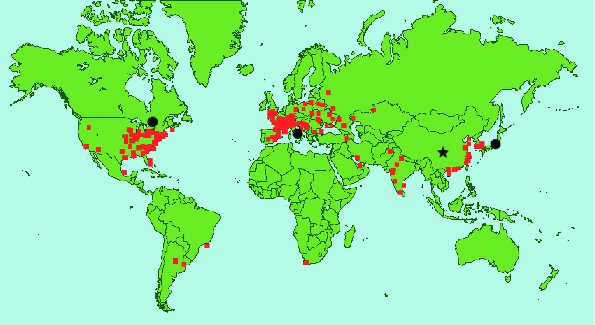
\includegraphics[width=1.0\textwidth]{figures/WorldMap.jpg}
    \caption{Location of China JinPing Underground Laboratory}
    \label{fig:cjpl}
\end{figure}
\end{minipage}
\begin{minipage}{.6\textwidth}
\begin{figure}[H]
    \centering
        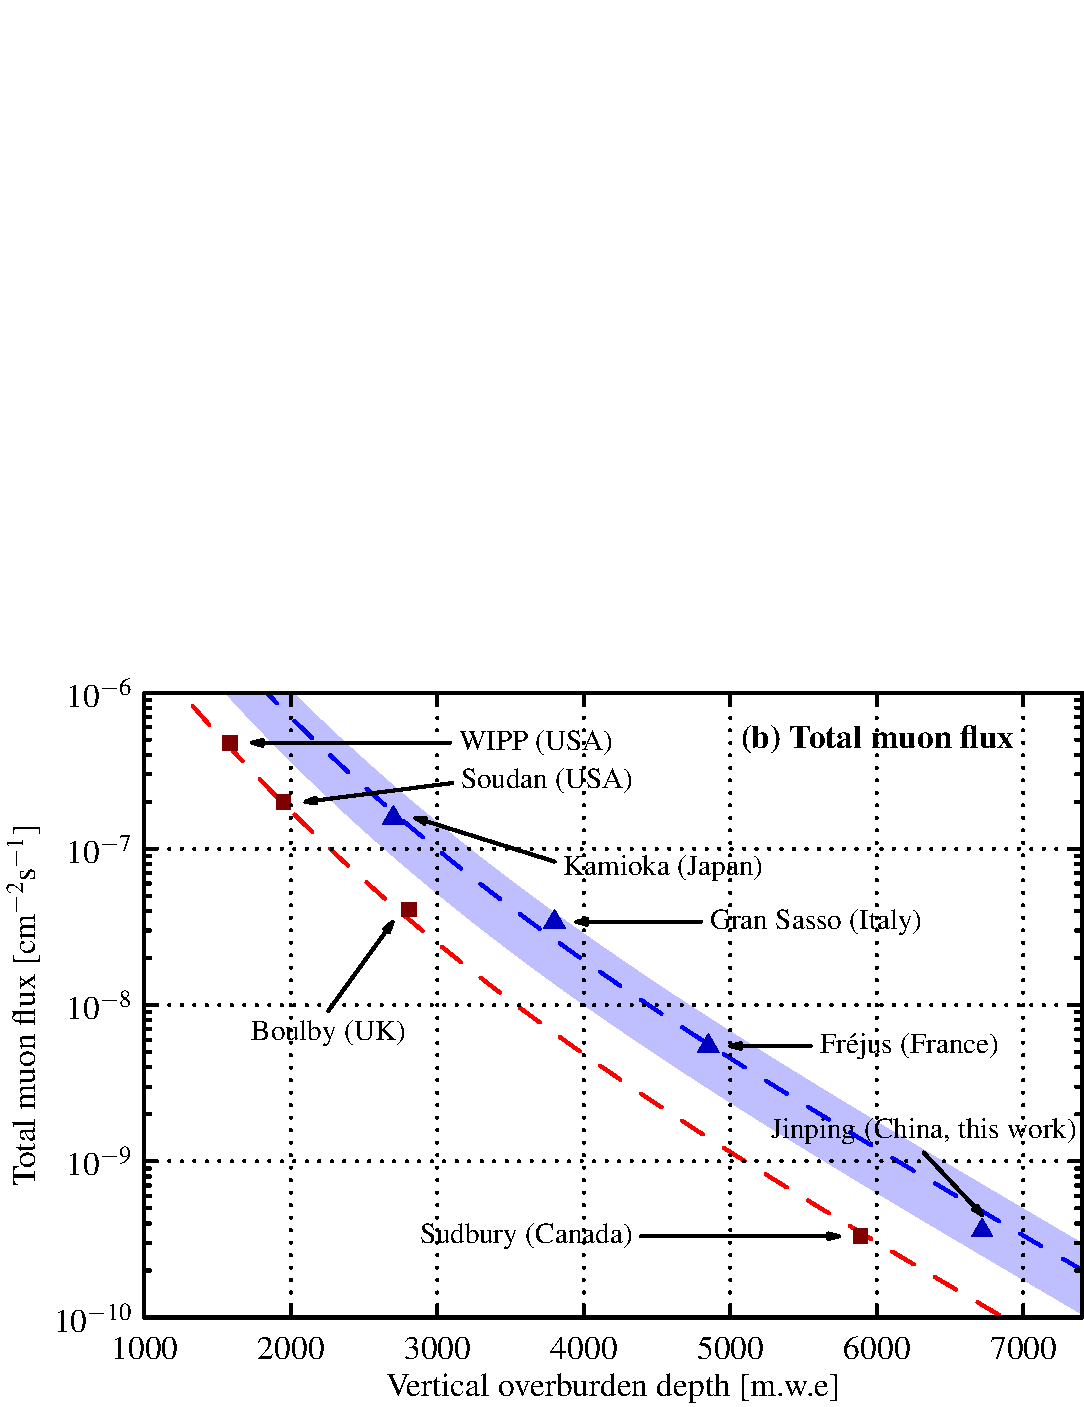
\includegraphics[width=1.0\textwidth]{figures/muonlab.pdf}
    \caption{Total intensity of $\mu$ at different underground sites}
    \label{fig:muon}
\end{figure}
\end{minipage}
\end{figure}

There is an ongoing 1ton prototype(Fig \ref{fig:1t}) in CJPL and next a hundred ton magnitude detector(Fig \ref{fig:100t}) will be built and an 5000 tons detector(Fig \ref{fig:1kt}) will be built in the future for Jinping Neutrino Experiment. 

\begin{figure}[H]
\begin{minipage}{.33\textwidth}
\begin{figure}[H]
    \centering
    \caption{1-ton prototype}
    \includegraphics[width=0.6\linewidth]{figures/prototype.jpeg}
    \label{fig:1t}
\end{figure}
\end{minipage}
\begin{minipage}{.34\textwidth}
\begin{figure}[H]
    \centering
    \caption{$\sim$100t detector}
    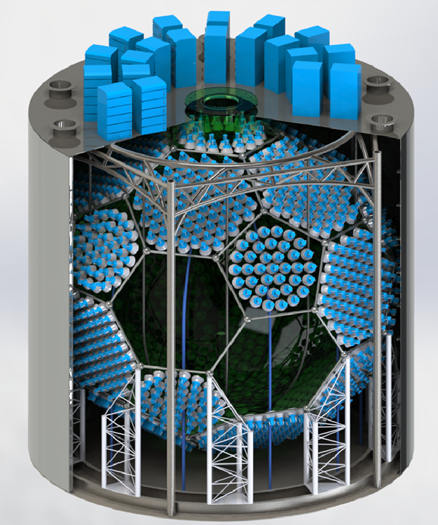
\includegraphics[width=0.6\linewidth]{figures/100tondetector.png}
    \label{fig:100t}
\end{figure}
\end{minipage}
\begin{minipage}{.33\textwidth}
\begin{figure}[H]
    \centering
    \caption{$\sim$5000t detector}
    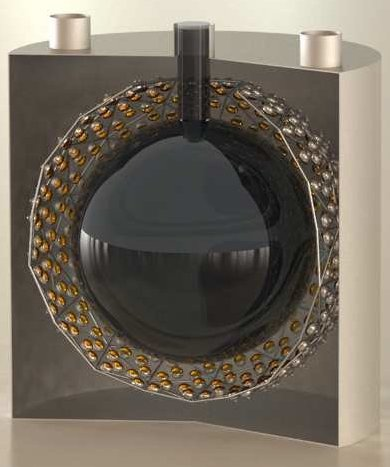
\includegraphics[width=0.6\linewidth]{figures/DetectoratJinping.jpg}
    \label{fig:1kt}
\end{figure}
\end{minipage}
\end{figure}

% section Jinping Neutrino Experiment (end)